\documentclass[12pt,a4paper]{article}
\usepackage[utf8]{inputenc}
\usepackage[spanish]{babel}
\usepackage{amsmath}
\usepackage{amsfonts}
\usepackage{amssymb}
\usepackage{makeidx}
\usepackage{graphicx}
\usepackage[left=2cm,right=2cm,top=2cm,bottom=2cm]{geometry}
\usepackage{float}
\usepackage{caption}
\usepackage{subfig}
\usepackage{enumitem}
\begin{document}
\begin{titlepage}

\centering

\includegraphics[scale=0.3]{UNC.PNG}

\vspace{1cm}
{\bfseries\LARGE Universidad Nacional de Córdoba \par}
\vspace{1cm}
{\scshape\Large Facultad de Matemática, Astronomía, Física y Computación\par}
\vspace{1cm}
{\scshape\Huge Trabajo Práctico N°2 de Redes Neuronales}
\vspace{1cm}

{\Large Chediack Ciminari, Camila }
\vspace*{0.3cm}


DNI: 41919762 \\


\vspace*{0.3cm}

E-mail:camila.chediack.c@mi.unc.edu.ar

\end{titlepage}

\begin{center}
\begin{large}
\textbf{El modelo de Izhikevich}
\end{large}
\end{center}

El modelo para una sola neurona debe ser computacionalmente sencillo y capaz de reproducir los patrones de disparo exhibidos por neuronas biológicas reales. El modelo de Hodking-Huxley es muy complicado del punto de vista computacional, dado que queremos reproducir el comportamiento de una sola neurona. Por otro lado, el modelo de integrate-and-fire es demasiado simple y por lo tanto incapaz de reproducir los picos y disparos exhibidos en una neurona cortical.  

A causa de la problemática planteada anteriormente, el \textit{modelo de Izhikevich} combina la dinámica biológica que reproduce el modelo Hodgkin-Huxley de una neurona junto con el modelo de integrate-and-fire, el resultado es un modelo que depende de cuatro parámetros: $a,b,c$ y $d$, y que puede reproducir los picos y disparos de distintos tipos de neuronas corticales, que son las que se encuentran en la corteza cerebral. 

Se trata de un sistema de dos ecuaciones diferenciales ordinarias de la siguiente forma:
\begin{align*}
v' &= 0.04v^2 + 5v +140 -u + I \\
u' &= a(bv-u)
\end{align*}
Con un reseteo auxiliar post-disparo:
$$v \geq 30 mV \Rightarrow \left\{ \begin{array}{l}
v \leftarrow c \\
u \leftarrow u+d
\end{array} \right.$$

La variable $v$ representa el potencial de membrana de la neurona mientras que $u$ es la variable que representa la recuperación de la membrana. El parámetro $a$ describe la escala de tiempo de recuperación de la membrana ($u$), valores más chicos significan una recuperación más lenta, un valor típico es $a=0.02$. El parámetro $b$ describe la sensibilidad de la recuperación de la membrana ($u$) con respecto a las fluctuaciones del subumbral del potencial de membrana\footnote{Con subumbral se refiere a cuando no se supera el umbral en el cual se dispara el potencial de acción}, el valor típico es $b=0.2$. Por último los parámetros $c$ y $d$, son los valores de reseteo post-disparo de la variable $v$ y $u$ correspondientes. 

Linealizando el sistema para obtener el polinomio característico nos da herramientas para conocer como es el comportamiento que tienen las variables, $u$ y $v$, entre sí. Dependiendo del valor que asuman los autovalores del polinomio característicos pueden tener un comportamiento de un punto de silla, espirables, órbitas, entre otros.

Primero se deben calcular los puntos estables del sistema, igualando a cero cada una de las ecuaciones del mismo de forma tal que nos queda:

\begin{align}
v' &= 0.04v^2 + 5v +140 -u + I = 0\\
u' &= a(bv-u) = 0
\end{align}
Despejando la ecuación (2) y reemplazando en (1) por su equivalente:
\begin{align*}
u &= b*v \\
0.04v^2 + (5-b)v + (140+I) &= 0
\end{align*}
Los valores que asume $u$ va a depender tanto de b y los dos valores que asume $v$, mientras que este último va a depender de los valores que asume $b$ e $I$. 

Armando la matriz Jacobiana de derivadas parciales de primer orden y calculando el determinante de esta menos el producto entre $\lambda$ y la matriz identidad:

$$det(J-I\lambda) =\begin{bmatrix}
&0.08v + 5- \lambda & -1 \\ \\
&ab & -a-\lambda
\end{bmatrix}$$

El polinomio característico va a ser: 
$$P(\lambda) = \lambda^2 +(a-0.08v-5)\lambda + (b-0.08v-5)*a = 0$$

En el análisis de cada uno de los casos posteriores se va a utilizar el polinomio, con sus correspondientes valores de variables y parámetros, para observar el comportamiento de $u$ con respecto a $v$ a través de los valores que asumen los autovalores.
\bigskip

\begin{center}
\begin{large}
\textbf{Comportamiento de las neuronas}
\end{large}
\end{center}

Considerando los valores comunes de los parámetros para $a$ y $b$ pero cambiando los valores a los cuales se resetean las variables $v$ y $u$ podemos representar el comportamiento de 3 clases distintas de neuronas corticales excitatorias. En la \textbf{Figura N°1}, el gráfico (a) corresponde a la neurona \textit{Regular Spiking (RS)}, con un valor bajo de reseteo para $v$ igual a $c=-65mV$ y un valor alto para $u$ igual a $d=8$. Luego de que se activa la corriente externa ($I(t)$) los primeros picos se disparan con un periodo de frecuencia más corto que el del resto de los picos. 


\begin{figure}[h!]
\centering
\caption*{\textbf{Figura N°1: Neuronas corticales excitatorias}}
\subfloat[\textit{RS}]{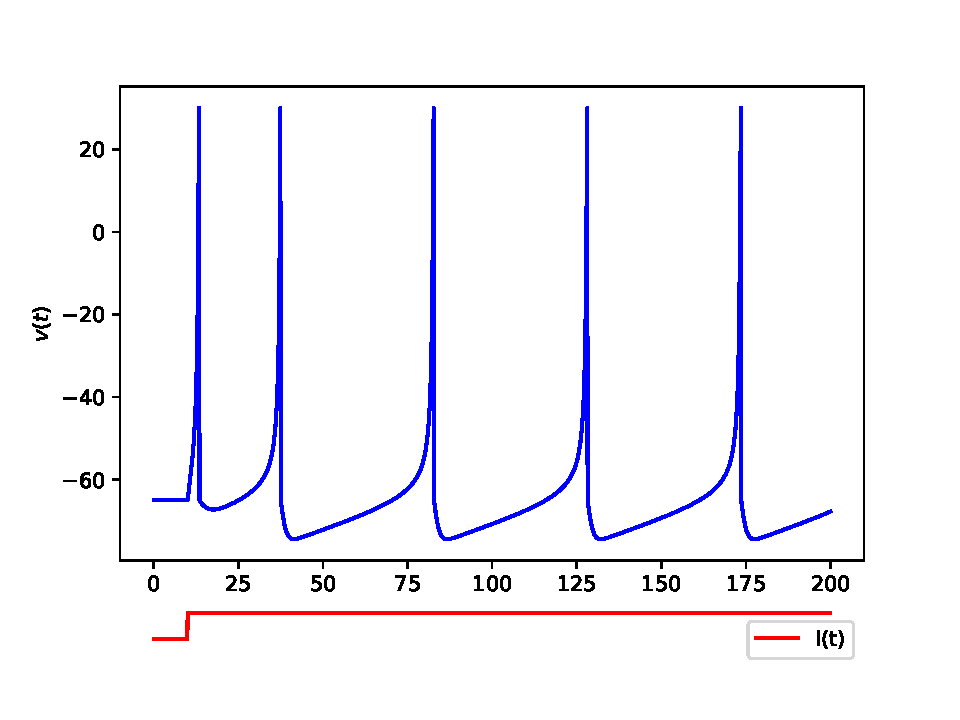
\includegraphics[scale=0.35]{RS.pdf}}
\subfloat[\textit{IB}]{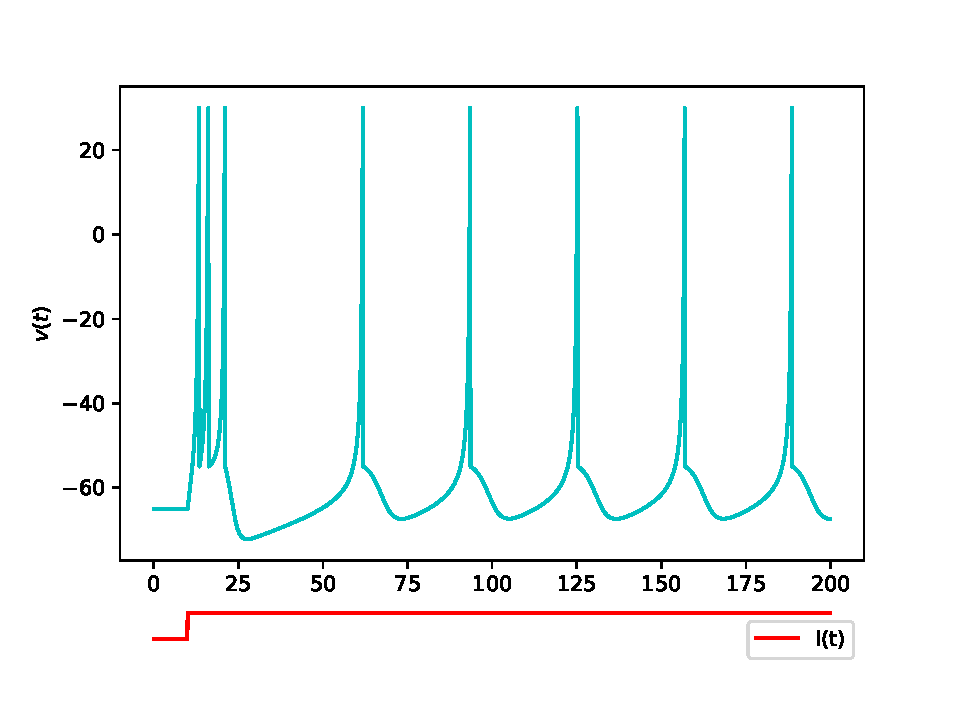
\includegraphics[scale=0.35]{IB.pdf}}
\subfloat[\textit{CH}]{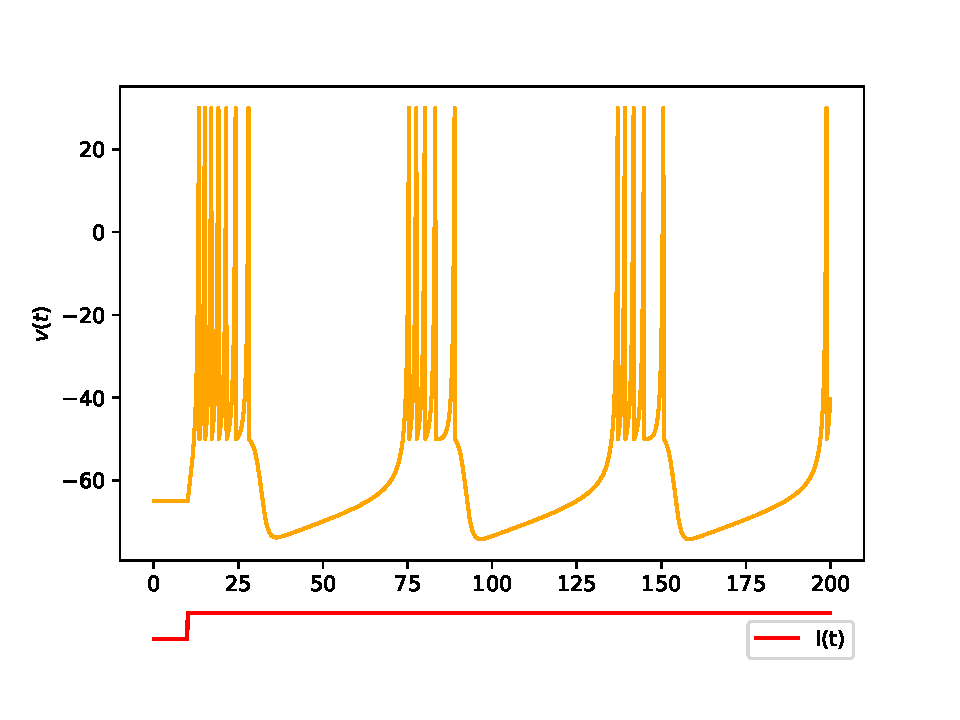
\includegraphics[scale=0.35]{CH.pdf}}
\end{figure} 

El gráfico (b) es la neurona \textit{Intrinsically bursting (IB)} con un alto valor de reseteo tanto para $v$ como para $u$ iguales a $c=-55mV$ y $d=4$. En el gráfico (c) se encuentra la neurona \textit{Chattering (CH)}  con la particularidad que son varios picos, distanciados entre ellos, donde en cada uno los disparos se realizan con gran frecuencia. El valor $c= -50 mV$ se considera un valor bastante alto de reseteo para el potencial de membrana y el parámetro $d=2$, un valor bastante moderado por lo que no afecta tan negativamente a $v$.

Por otro lado tenemos dos clases de células corticales inhibitorias, las neuronas \textit{Fast Spiking (FS)}, que al tener una rápida recuperación, dado por el parámetro $a=0.1$, se disparan potenciales de acción con una altísima frecuencia, como se puede visualizar en el primer gráfico de la \textbf{Figura N°2}. La otra clase son las neuronas \textit{Low-Threshold Spiking (LTS)} que también disparan potenciales de acción con alta frecuencia pero, a diferencia de las anteriores, después de un cierto periodo esta frecuencia disminuye. Esto se debe a que le corresponde un valor de $b=0.25$, mientras más alto sea este valor resulta en mayores oscilaciones antes de superar el umbral y con picos de umbral bajos. Este tipo de neurones tiene una despolarización de membrana baja y negativa.

\begin{figure}[h!]
\centering
\caption*{\textbf{Figura N°2: Neuronas corticales inhibitorias}}
\subfloat[\textit{FS}]{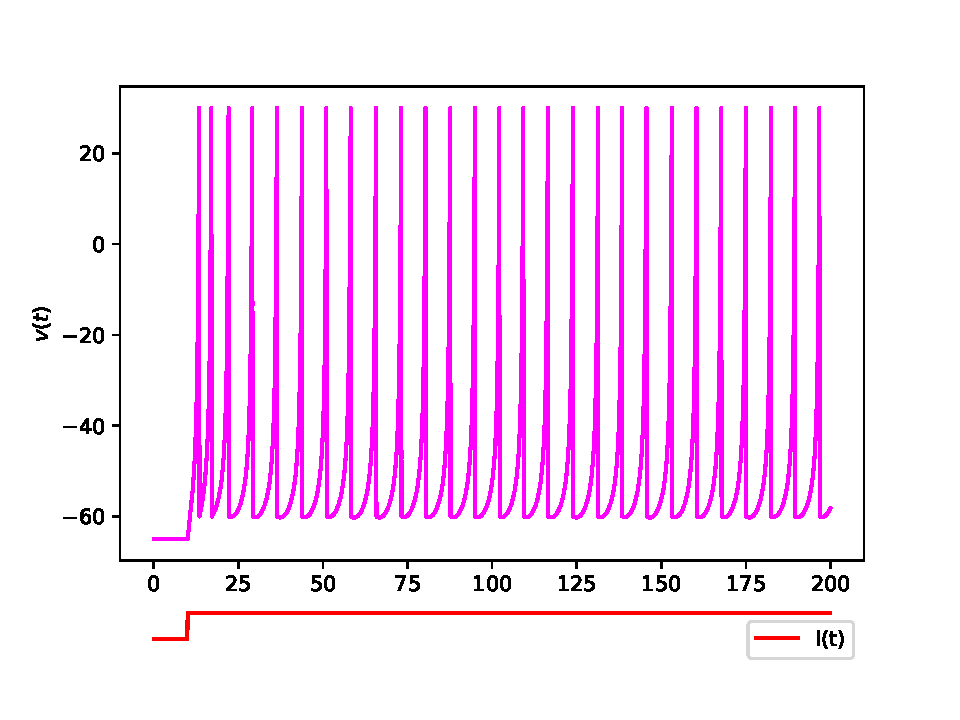
\includegraphics[scale=0.55]{FS.pdf}}
\subfloat[\textit{LTS}]{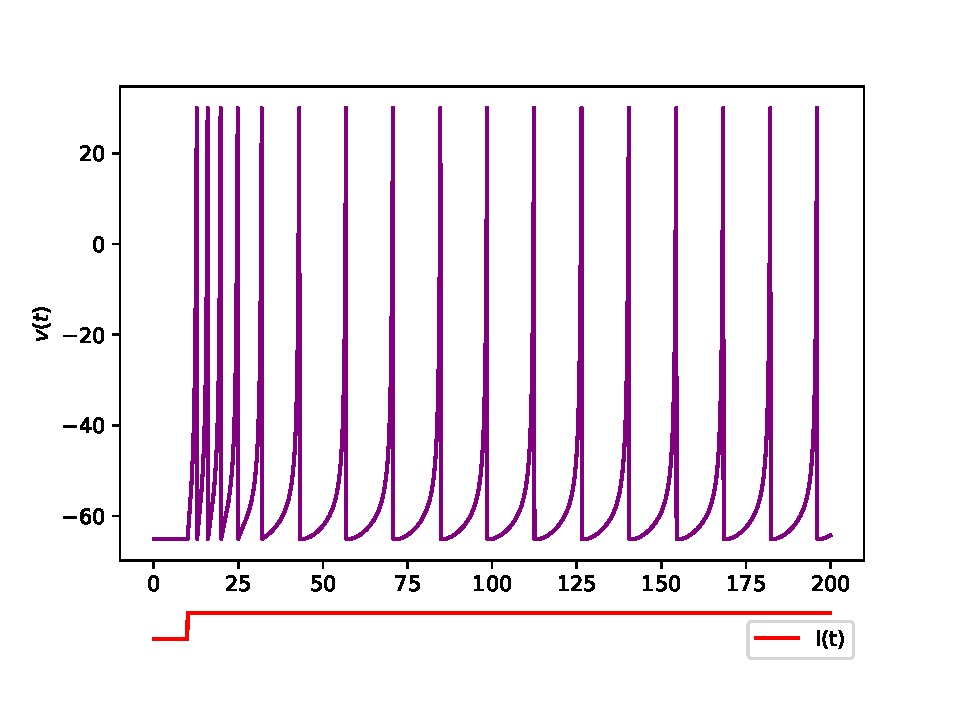
\includegraphics[scale=0.55]{LTS.pdf}}
\end{figure}
 
Este modelo también puede reproducir las neuronas \textit{Thalamo-Cortical}, que son justamente aquellas que se encuentran en el tálamo. En estas se producen dos disparos, uno cuando la membrana se encuentra en su potencial de reposo alrededor de $-60mV$ y otro cuando recibe una corriente negativa que hace que se hiperpolarice, llegando alrededor de los $-90mV$. En el primer caso vemos que después del disparo tiene un comportamiento similar al de las neuronas \textit{RS} pero con picos menos frecuentes. En el segundo caso vemos que después de la hiperpolarización, el disparo hace que se generen varios potenciales de acción con bastante frecuencia hasta que se estabiliza, para ello se estableció un valor de $b$ bastante chico, lo cual baja las fluctuaciones del potencial de membrana antes de llegar al umbral. Esto se puede apreciar en la \textbf{Figura N°3}, donde la imagen de la izquierda corresponde al primer disparo y la de la derecha es después de la hiperpolarización. 

\begin{figure}[H]
\centering
\caption*{\textbf{Figura N°3: Neurona \textit{Thalamo-cortical}}}
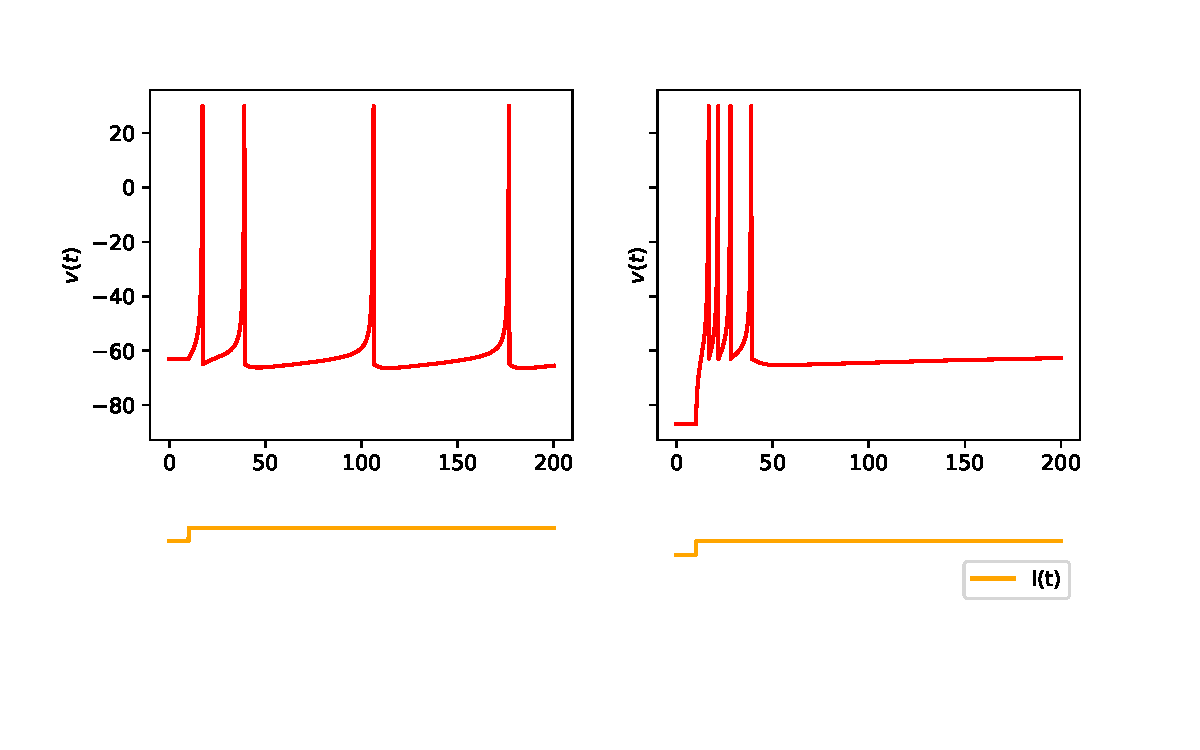
\includegraphics[scale=0.70]{TC2.pdf}
\end{figure}

Existen otros tipos de neuronas cuya dinámica se puede reproducir a través del \textit{modelo de Izhikevich}, en particular se tiene la neurona \textit{Resonator (RZ)}, con oscilaciones sostenidas del subumbral del potencial de membrana. A través de un pequeño impulso de la corriente, la neurona sale de su estado de reposo y aparecen picos con una cierta frecuencia, como se ve en la \textbf{Figura N°4}. Este comportamiento corresponde a un parámetro $a = 0.1$ (una recuperación rápida de $u$) y un $b \approx 0.26$ (mientras mayor sea mayores son las fluctuaciones del subumbral del potencial de membrana). Al principio se utiliza un $b$ levemente menor y una corriente externa $I = 0.016$ para generar las fluctuaciones y que no se produzca un potencial de acción. Luego se aumenta la corriente a $I = 0.03$, valor para el cual se produce un potencial de acción con picos que no son demasiado frecuentes. 

\begin{figure}[h]
\caption*{\textbf{Figura N°4: Neurona \textit{Resonator}}}
\centering
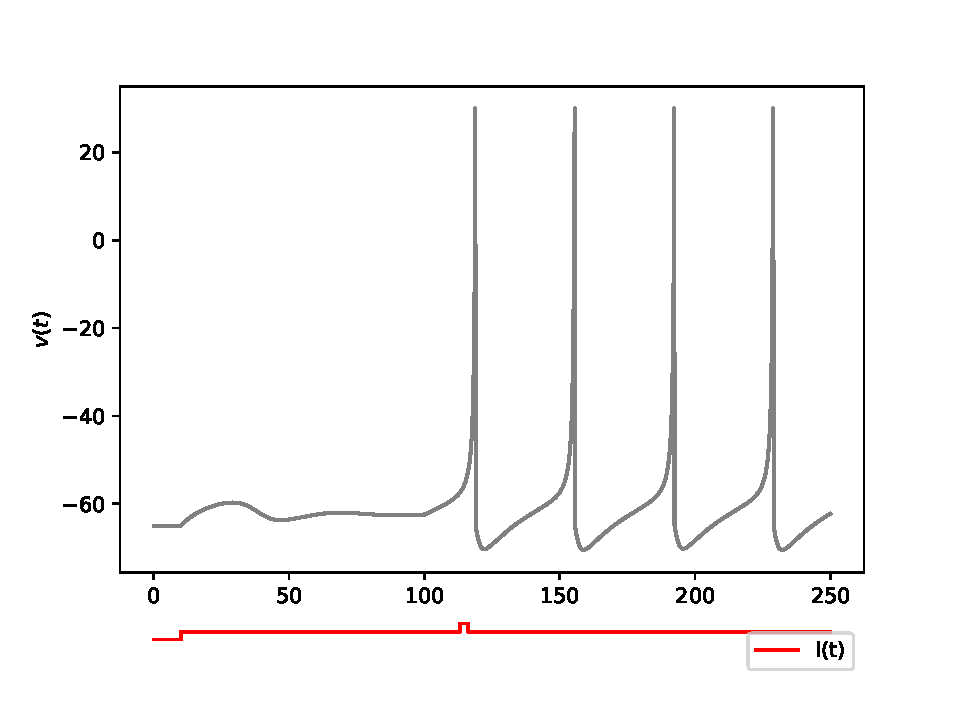
\includegraphics[scale=0.7]{RZ.pdf}
\end{figure}

Utilizando el polinomio característico, se calcularon los autovalores para cada tipo de neurona, en todas las ocasiones exceptuando por el último tipo (la neurona Rezonator) se obtuvieron autovalores negativos y no hubo convergencia del sistema hacia su punto fijo, posiblemente se debe a que los valores iniciales están lejos del mismo. A su vez los puntos fijos dependen de los parámetros que van cambiando en cada caso.

En cuanto a la neurona Rezonator se hallaron autovalores complejos conjugados, donde la parte real es negativa, por ello se ve un comportamiento de espiral descendente hacia el centro. 

\begin{tabular}{ccc}
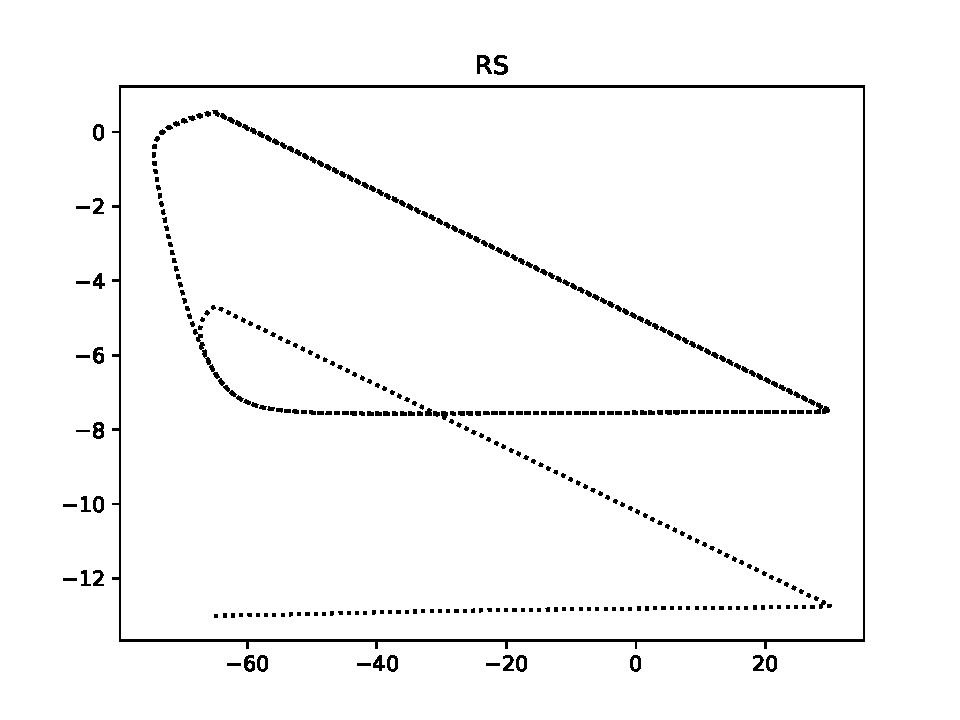
\includegraphics[scale=0.3]{RSvu.pdf} 
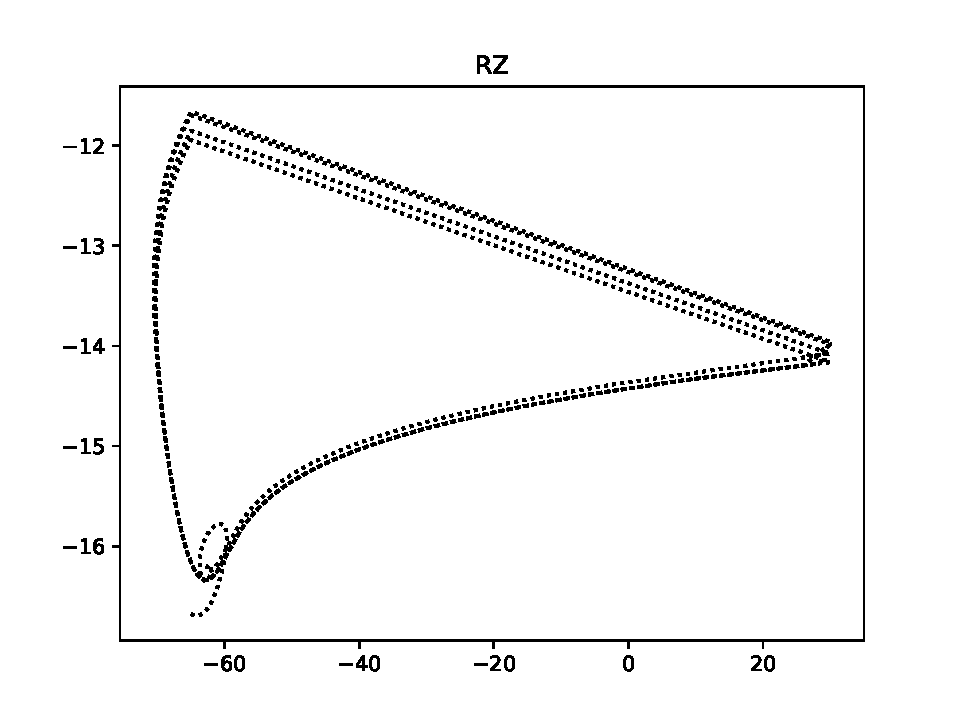
\includegraphics[scale=0.3]{RZuv.pdf} 
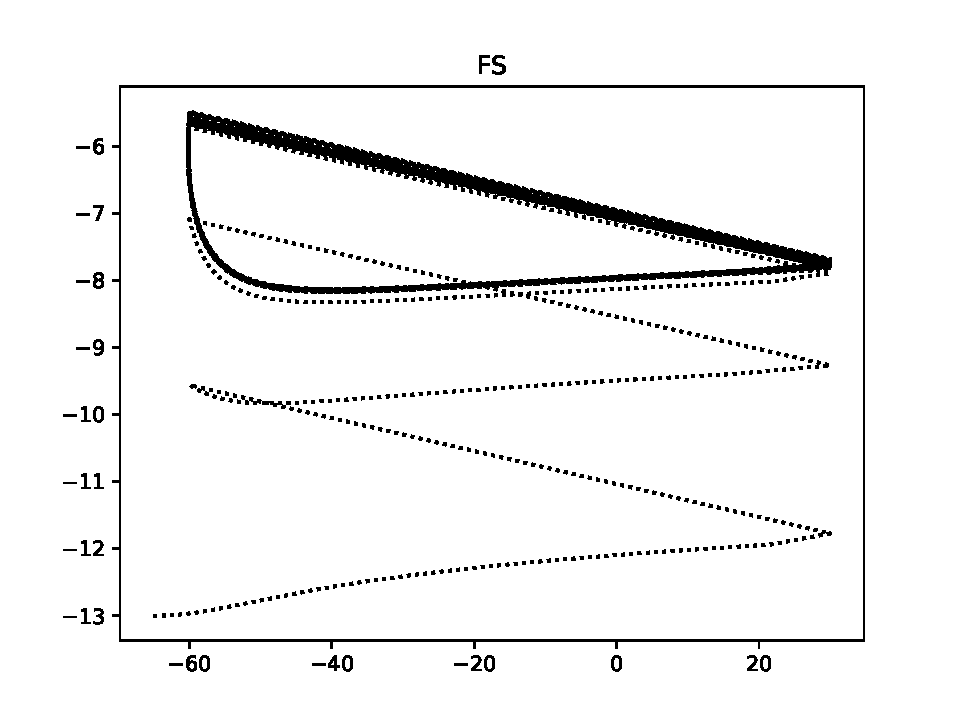
\includegraphics[scale=0.3]{FSuv.pdf} \\
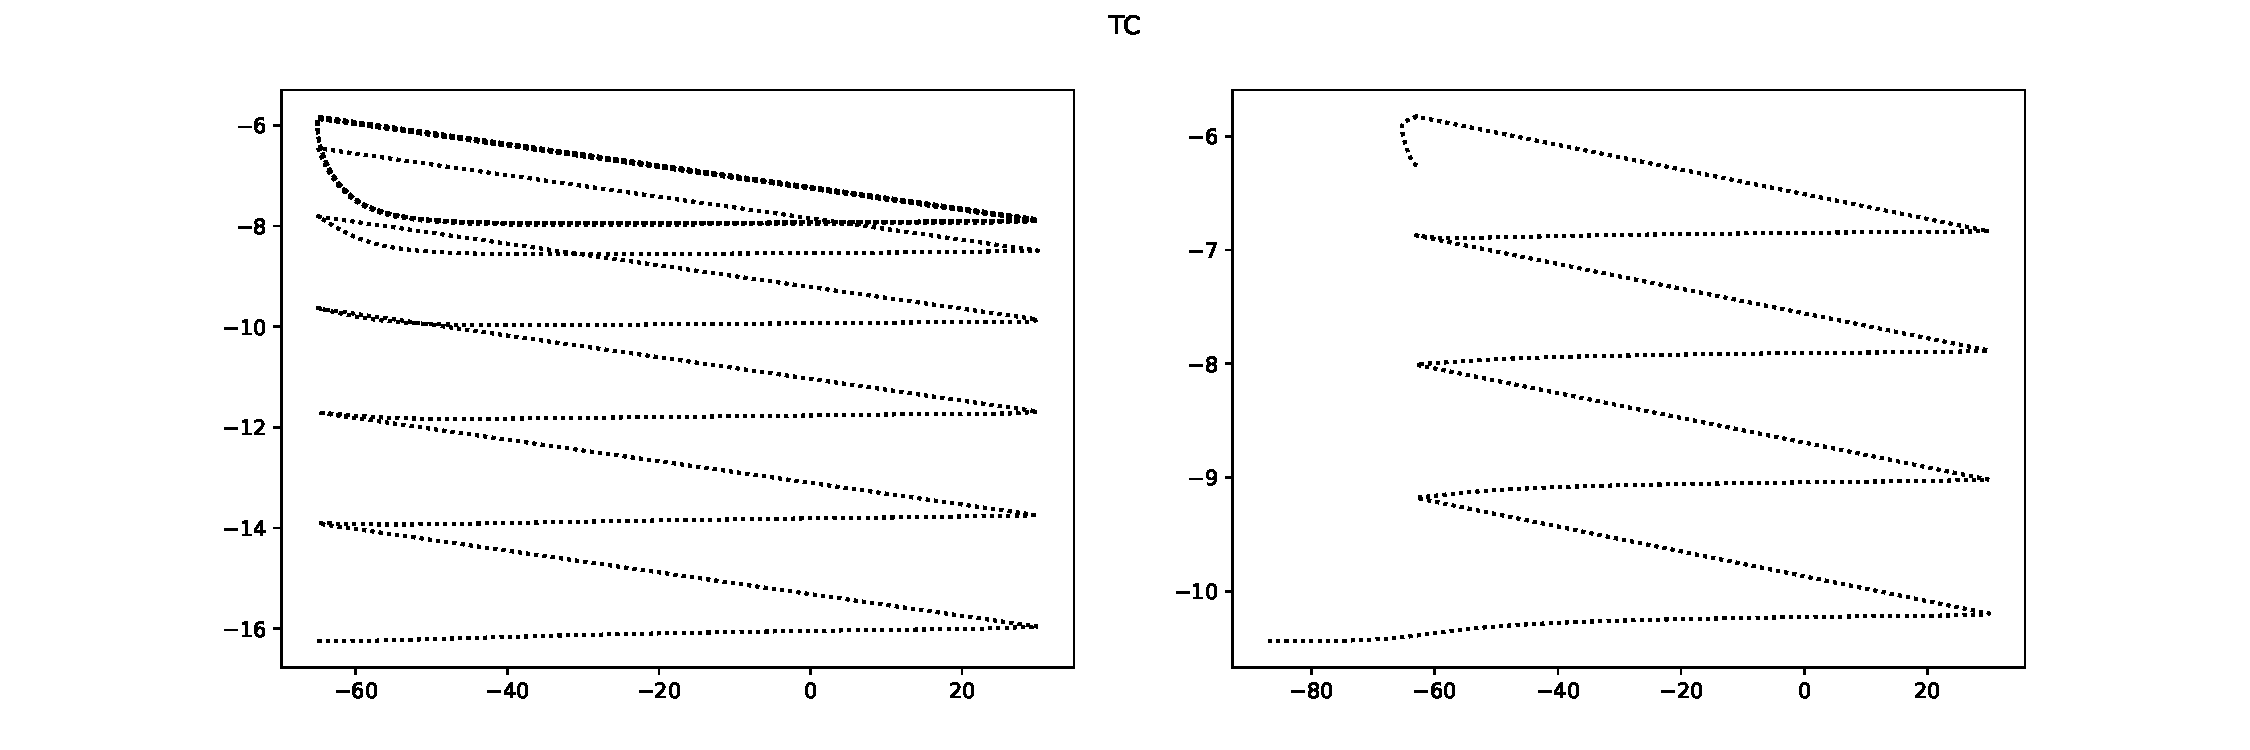
\includegraphics[scale=0.3]{TCuv.pdf}
\end{tabular}
\end{document}